\documentclass[a4paper, 10 pt, conference]{hsmrw} 
\usepackage[utf8]{inputenc}
\IEEEoverridecommandlockouts                       
\overrideIEEEmargins
\usepackage{mathtools}
\usepackage{geometry}
\geometry{
    a4paper,
    left=20mm,
    right=20mm,
    top=25mm,
    bottom=25mm,
}
\usepackage[labelsep=space]{caption}
\usepackage{newtxmath,newtxtext}
\usepackage{authblk}
\usepackage{pgfplots}
\usepackage{graphicx}
\usepackage[colorlinks,urlcolor=blue]{hyperref} 
\urlstyle{same}
\usepackage{newtxtext,newtxmath}

\setlength{\parindent}{0pt}

\pgfplotsset{compat=newest} 
 
\title{\LARGE \bf
Technical Paper Format for the Hamlyn Symposium on Medical Robotics} 

\author{\LARGE A. N. Author$^{1}$}
\author{\LARGE A Co-author$^{1}$} 
\author{\LARGE B Co-author$^{2}$} 

\affil{\Large\textit{$^{1}$Institute for xxx, University XXX,}\\ \Large\textit{$^{2}$Institute for xxx, University Hospital XXX}\\ \Large\textit{a.n.author@abc.edu}}

\begin{document}

\maketitle
\thispagestyle{empty}
\pagestyle{empty}

\section*{INTRODUCTION}
The Hamlyn Workshop on "Open-Source Software in Surgical, Biomedical and AI Technologies" is held at the Royal Geographical Society. Conveniently located in the heart of central London, the symposium venue is within a close proximity to the landmarks, museums and Royal parks of London. 

\section*{MATERIALS AND METHODS}
Topics to be addressed by the workshop include, but are not limited to: (1) Open-source software/hardware libraries and frameworks for surgical and biomedical sciences (2) Open-source AI solutions for surgical and biomedical sciences (3) Open-source software/hardware regulations in clinical sciences (4) Maintaining and supporting surgical and biomedical software/hardware (5) Incorporating open-source software/hardware in clinical trials (6) Open-source software/hardware solutions for low to middle-income countries (7) Case studies showcasing novel applications and combinations of existing open-source software and hardware, and (8) Project summaries, methodological approaches, research findings, and initiatives related to Open-Source Software for Surgical Technologies.


\section*{RESULTS}
Your submission should be no more than 2 pages to include the following sections: INTRODUCTION, MATERIALS AND METHODS, RESULTS, DISCUSSION and REFERENCES.
\begin{itemize}
    \item \textbf{Length:} Maximum of A4 2 pages;
    \item \textbf{Paper size:} DIN A4 Size (210 mm x 297 mm);
    \item \textbf{Rand:} Leave a 25mm margin at top and bottom of the page, and a 20mm margin at left and right sides;
    \item \textbf{Page-Layout:} Set the text in two columns of 80 mm width, with a central separation of 10mm;
    \item \textbf{Font properties and size:} Title: 14 pt, bold; Authors: 14 pt, normal; Institute + E-mail address: 12 pt, italics; Section headings: 10 pt, Capitals, bold; Text: 10 pt, normal; Figure captions and references: 9pt, normal.
\end{itemize}

\begin{figure}[t]
\centering
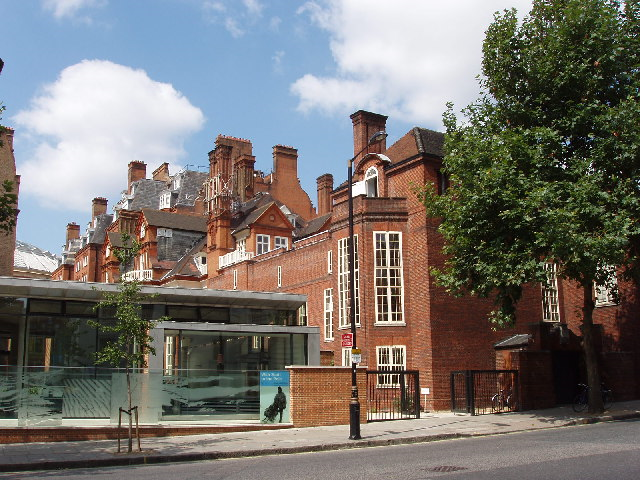
\includegraphics[width=\columnwidth]{examplefig.png}
\caption{Founded in 1830, the Royal Geographical Society is a world centre for geography: supporting research, education, expeditions and fieldwork, and promoting public engagement and informed enjoyment of the world.}
\label{fig_example}
\end{figure}

\section*{DISCUSSION}
Completed papers should be submitted as a pdf-file via the online submission at: \url{https://openreview.net/group?id=hamlynsymposium.org/Hamlyn_Symposium/2025/Workshop/OSS_in_SurgTech#tab-recent-activity}

Please contact the following e-mail address with any questions: \href{mailto:s.chopra@ucl.ac.uk}{s.chopra@ucl.ac.uk} 

\nocite{*}
\bibliographystyle{IEEEtran}
\bibliography{hsmrw}

\end{document}
